\documentclass[10pt, landscape]{article}
\usepackage[scaled=0.92]{helvet}
\usepackage{multicol}
\usepackage{calc}
\usepackage{ifthen}
\usepackage[landscape]{geometry}
%\usepackage{hyperref}

\usepackage{newtxtext} 

%for strikeout
\usepackage{ulem}

%For editing parbox
\usepackage[table]{xcolor}
%For editing itemise margins, reduce iterm separaion and list separation
\usepackage{enumitem}
% For math
\usepackage{amsmath,amsthm,amsfonts,amssymb}

%For pictures / figures
\usepackage{color,graphicx,overpic}
\graphicspath{ {./images/} }

%\usepackage{newtxtext} 
%\usepackage{amssymb}
%\usepackage[table]{xcolor}
%\usepackage{vwcol}
%\usepackage{tikz}
%\usepackage{wrapfig}
%\usepackage{makecell}

\pdfinfo{
  /Title (CS2107-notes.pdf)
  /Creator (Ger Teck)
  /Author (Ger Teck)
  /Subject ()
  /Keywords (tex)}

%% Margins for PAPER

% This sets page margins to .5 inch if using letter paper, and to 1cm
% if using A4 paper. (This probably isn't strictly necessary.)
% If using another size paper, use default 1cm margins.
\ifthenelse{\lengthtest { \paperwidth = 11in}}
	{ \geometry{top=.3in,left=.3in,right=.3in,bottom=.3in} }
	{\ifthenelse{ \lengthtest{ \paperwidth = 297mm}}
		{\geometry{top=0.5cm,left=0.5cm,right=0.5cm,bottom=0.5cm} }
		{\geometry{top=0.5cm,left=0.5cm,right=0.5cm,bottom=0.5cm} }
	}

% Turn off header and footer
\pagestyle{empty}
% for tight centres (less spacing)
\newenvironment{tightcenter}{%
  \setlength\topsep{0.5pt}
  \setlength\parskip{0.5pt}
  \begin{center}
}{%
  \end{center}
}

% Redefine section commands to use less space
\makeatletter
\renewcommand{\section}{\@startsection{section}{1}{0mm}%
                                {-1ex plus -.5ex minus -.2ex}%
                                {0.5ex plus .2ex}%x
                                {\normalfont\large\bfseries}}
\renewcommand{\subsection}{\@startsection{subsection}{2}{0mm}%
                                {-1explus -.5ex minus -.2ex}%
                                {0.5ex plus .2ex}%
                                {\normalfont\normalsize\bfseries}}
\renewcommand{\subsubsection}{\@startsection{subsubsection}{3}{0mm}%
                                {-1ex plus -.5ex minus -.2ex}%
                                {1ex plus .2ex}%
                                {\normalfont\small\bfseries}}
% change font
%\renewcommand{\familydefault}{\sfdefault}
%\renewcommand\rmdefault{\sfdefault}
\linespread{1.05}

\makeatother

% Define BibTeX command
\def\BibTeX{{\rm B\kern-.05em{\sc i\kern-.025em b}\kern-.08em
    T\kern-.1667em\lower.7ex\hbox{E}\kern-.125emX}}

% Don't print section numbers
\setcounter{secnumdepth}{0}

\setlength{\parindent}{0pt}
\setlength{\parskip}{0pt plus 0.5ex}

%% this changes all items (enumerate and itemize, reduce margins) ITEMIZE SEPARATION HERE
\setlength{\leftmargini}{0.5cm}
\setlength{\leftmarginii}{0.5cm}
\setlist[itemize,1]{leftmargin=2mm,labelindent=1mm,labelsep=1mm, itemsep = 0mm}
\setlist[itemize,2]{leftmargin=4mm,labelindent=1mm,labelsep=1mm, itemsep = 0mm}

%itemsep = 0mm
%\setlist{nosep}

% -------------------------------------------------------------------------------

% START OF DOCUMENT HERE

\begin{document}
\raggedright
\footnotesize
\begin{multicols*}{3}

% multicol parameters
% These lengths are set only within the two main columns
%\setlength{\columnseprule}{0.25pt}
\setlength{\premulticols}{1pt}
\setlength{\postmulticols}{1pt}
\setlength{\multicolsep}{1pt}
\setlength{\columnsep}{2pt}

%% DOCUMENT NAME HERE
\begin{center}
     \Large{\textbf{CS2107 Intro Information Security}} \\
\end{center}
AY23/24 Sem 2, github.com/gerteck


\section{0. Introduction}
CS2107: Introductory module, illustrates fundamentals of how systems fail due to malicious activities and how they can be protected. 

\textbf{Lecture Notes notation}
\begin{itemize}
\item \textbf{Textbook:} Security in Computing (5th ed). Prentice Hall. Reference [PFx.y] refer to chapter x section y of this book.
\item Links with ``read'': Part of lecture, required. 
\item Links with ``see'': Optional good to browse references.
\end{itemize}

\subsection{Internet Security Threat Report Exc. Summary}
Persistent threats are threats that often operate within the shadows, outside of attention focused. 
\begin{itemize}
\item Highly targeted, often use combination of social engineering and software vulnerabilities to establish footholds within the targeted enterprise.
\item Network protection not enough to migitgate threats, comprehensive monitoring program required to scan all internal and external network traffic. Identifying, securing data is also key to protecting assets.
\item Recent attack types: Formjacking, Ransomware, Living off the Land (LotL), 
\end{itemize}


\subsection{Introduction to Computer/Info Security}
Systems may fail due to operator mistakes, hardware failures, poor implementation etc. Many systems robust against typical noise. Security is about intentional failures inflicted by deliberate human actions. \\
\textbf{Security Definitions:} C-I-A triad
\begin{itemize}
\item \textbf{Confidentiality}: Prevention of unauthorized disclosure of information.
\item \textbf{Integrity}: Prevention of unauthorized modification of info / processes.
\item \textbf{Availability}: Prevention of unauthorized withholding of info / resources.
\item Other requirements may include (Confidentiality: anonymity, covert channel), (Integrity: Non-repudiation (digital signature)), (Other: Accountability, traitor-tracing (printout w hidden watermark)) etc.
\item Importance of understanding security requirements before adopting mechanisms. Do not adopt mismatched protection mechanisms.
\end{itemize}

\subsubsection{Difficulties in achieving Security}
\begin{itemize}
\item \textbf{Security not considered} (in early design stage). \\
Lack of adverarial thinking in design / trade-off in security with ease-of-use, performance / cost.
\item Difficult to formulate requirements /design / implementation bugs. 
\item Difficult to operate/manage (Human error). \\
\item \textbf{Known Vulnerabilities: CVE (Common vulnerabilities \& Exposures}. Repository of discovered vulnerabilities. Significant portion considered "implementation bugs".
\item \textbf{Zero-day Vulnerabilities}: Unpublished vulnerabilities. If attackers deploy attacks on zero-day v., victims have "zero-day" to react. Not easy to get.
\end{itemize} 


\section{1. Encryption}

% To update:
\textbf{Key Summary \& Takeaways}
\begin{itemize}
\item \textbf{Encryption designed for confidentiality.} (Not necessarily integrity).
\item Formulate attack scenario by defining attacks it can prevent. 
\item Notions of "Oracle": Encryption, Decryption, Padding Oracle.
\item \textbf{Key strength}: Quantifying security by equivalence of best-known attack to exhaustive search.
\item No known efficent attacks on modern schemes under "original" threat models, but there are pitfalls. Such as implementation error (wrong mode, wrong random source, mishandle of IV), side channel attack, implicity require integrity, padding oracle attack.
\item Design of various symmetric key encryption schemes:
	\begin{itemize}
	\item One-time pad, stream cipher (xor'ing with "pseudo-random" string)
	\item Block cipher (mode of operations: CBC, ECB, CTR, GCM)
	\end{itemize}
\item \textbf{Crucial role of IV}. (Need randomness for indistinguishability). Make encryption probabilistic, how it is deployed, why it is important.
\end{itemize}

\subsubsection{Definitions}
\begin{itemize}
\item \textbf{Symmetric Key Encryption Scheme}: Two algorithms: encryption and decryption. Meets correctness property, and must be secure.
\item \textbf{Correctness:} $(D_k (E_k (x) ) = x )$. \textbf{Security}: Informally, "difficult" to derive useful info of the key k, and plaintext x. Ciphertext resemble random sequence of bytes.
\item \textbf{Cryptography}: Study of techniques in securing communication in present of adversaries with access. Encryption just a primitive (other includes crypto hash, digital signature etc. Common placeholders: Alice, Bob, Eve ("eavesdroppper"), Mallory (malicious, modify message), etc.
\end{itemize}

\subsubsection{Attack Model}
\textit{Aka: Threat / Adversary / Security Model, Attack Scenario.} \\
Measuring \textbf{security of a system}: Through attack classes it can prevent. Secure w.r.t these classes of attacks. Attack models are application-dependent. Attack models described by:
\begin{itemize}
\item Attacker's knowledge (info / service exposed) and computing resources
\item Attacker's goal
\end{itemize}
\textbf{Types of information we assume access to:} (Access to info can be formulate to accesses to an \textbf{"Oracle"}).
\begin{itemize}
\item \textbf{Ciphertext only attack:} Adversary given collection of ciphertext c. May know some properties 
of the plaintext, for e.g. the plaintext is an English sentence. (adv. can’t choose plaintext).
\item \textbf{Known plaintext attack:} Adversary given collection of plaintext m and corresponding ciphertext c. (adv. can’t choose plaintext.)
\item \textbf{Chosen plaintext attack (CPA):} Access to blackbox (i.e. the oracle). \\
Can choose, feed any plaintext m, obtain corresponding ciphertext c (all encrypt with the same key), reasonable large number of times. Can see ciphertext and choose next input.  \textit{(black-box called encryption oracle).}
\item \textbf{Chosen ciphertext attack (CCA2)}: Same as chosen plaintext attack, but adv. chooses ciphertext and blackbox outputs plaintext. \textit{black-box called decryption oracle}. \\
\textbf{Note}: (strange to assume attacker has power to decrypt, but good reason is that in some practical scenario, attacker does have some but not full decryption capability, e.g. \textit{padding oracle}. To cater for all scenarios, in formulation and design of encryption, we consider oracle with full decryption capability.)
\end{itemize}

\subsubsection{Adversary's Goals}
\begin{itemize}
\item \textbf{Total Break}: Attacker wants to find the key.
\item \textbf{Partial Break}: Few definitions, e.g. decrypt ciphertext, determine coarse information about plaintext, etc.
\item \textbf{Indistinguishability (IND)}: ) Attacker may satisfy with distinguishability of ciphertext: with some “non-negligible” probability more than ½, the attacker is able to distinguish the ciphertexts of a given plaintext (say, “Y”) from the ciphertext of another given plaintext (say, “N”). (Equivalently, unable to distinguish the ciphertext and a randomly sequence).
\item \textbf{Note}: total break most difficult goal, since achieves all. Distinguishability weakest goal, design cryptosystem preventing weakest goal.
\end{itemize}

\subsection{Classicial Ciphers}
\begin{itemize}
\item \textbf{Substitution Cipher} 
	\begin{itemize}
	\item \textbf{Plaintext, ciphertext}: String over a set of symbols U.
	\item \textbf{Key}: Subsitution table S, 1-1 onto function from U to U.
	\item \textbf{Key space}: Set of all possible keys (e.g. 27). \textbf{Space Size} is total number of possible keys (factorial, 27!). \textbf{Key Size} is number of bits required to represent a key. (log 2 (27!), since 27! unique) 
	\item \textbf{Exhaustive Search (Brute-force): Can be infeasible in worst case}
	\item \textbf{Known-plaintext-attack}: Access to pairs of ciphertext and corresponding plaintexts: \textit{Sub. cipher “not secure / totally broken under known plaintext attack”}. (Possible in practice, e.g. certain words in header of email "From, Subject", protocols bytes fixed header information etc.)
	\item \textbf{Ciphertext only attack}: Vulnerable to frequency analysis attack, when plaintexts English sentences.
	\end{itemize}
\item \textbf{Permutation Cipher}, aka transposition cipher
	\begin{itemize}
	\item Groups plaintext into blocks of $t$ characters, applies secret permutation (1-1 onto function). Fails miserably on known-plaintext attack.
	\centerline{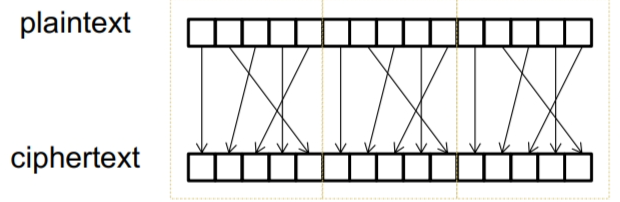
\includegraphics[width=0.4\linewidth]{permutationCipher}}
	\end{itemize}
\item S \& P cipher not secure, performing substitution multiple times no use. However, by interlacing them (S\&P), attacks become more difficult. Many modern encryption scheme (e.g. AES) designed using rounds of S \& P.
\item \textbf{One Time Pad}


\end{itemize}























\end{multicols*}
\end{document}
